\subsection{\bt}
\label{sec:bt}

\subsubsection{Wprowadzenie}

\bt{} to własnościowy standard komunikacji bezprzewodowej. Korzystając
z~połączenia \bt{} możliwe jest tworzenie sieci PAN --- \emph{Personal Area
Network}.

Sieci PAN oparte o~\bt{} pozwalają na połączenie maksymalnie 8 urządzeń
w~konfiguracji klienci\dywiz serwer \cite{wiki:pan}. W~sieci występuje jeden
serwer i~wszyscy klienci powinni znajdować się w~jego zasięgu. Możliwe jest
także zwiększenie zasięgu sieci poprzez węzły pośrednie (tzw.
\emph{scatternet}) \cite{bt}.

\begin{figure}[h!]
  \centering
  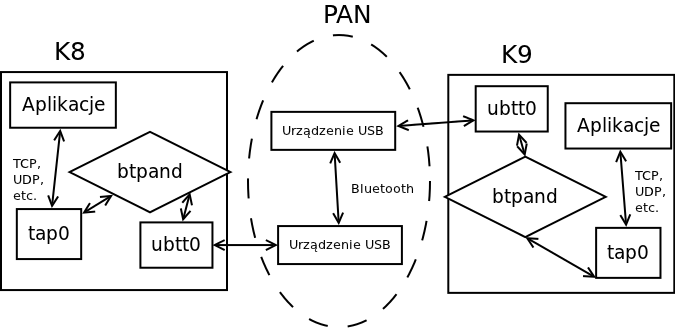
\includegraphics[width=\textwidth]{figury/bluetooth/schemat.png}
  \caption{Schemat ideowy naszej konfiguracji połącznia \bt.}
\end{figure}

W systemie \bsd, połączenia w tej technologii można realizować za pomocą
wirtualnego urządzenia \texttt{tap}, na które demon \texttt{btpand}
przekierowuje pakiety.

\subsubsection{Konfiguracja połączenia}

Na maszynie laboratoryjnej załadowano niezbędne sterowniki do obsługi
urządzenia \bt. Postąpiliśmy zgodnie z~instrukcjami podanymi po wywołaniu
skryptu \texttt{sterowniki -b}.

\begin{lstlisting}
% sudo kldload uhci ehci ng_ubt
\end{lstlisting}

Są to sterowniki odpowiedzialne za stos USB oraz samo urządzenie \bt,
podłączone do komputera przez USB. Bezpośrednio po załadowaniu sterowników
urządzenie nie było widoczne w komunikacie polecenia \texttt{sudo lsusb}. Po
odłączeniu i~ponownym podłączeniu, urządzenie zostało wykryte:

\begin{lstlisting}[caption={Potwierdzenie w logu systemowym, że urządzenie \bt{} zostało wykryte.}]
% dmesg | tail
ugen4.2: <ZyDAS> at usbus4
ugen1.2: <Logitech> at usbus1
ugen0.2: <vendor 0x0a12> at usbus0^
ubt0: <vendor 0x0a12 product 0x0001, class 224/1, rev 1.10/3.73, addr 2> on usbus0
\end{lstlisting}

Po upewnieniu się, że urządzenie zostało poprawnie rozpoznane, zgodnie
z~wcześniejszą instrukcją uruchomiliśmy usługę \bt.

\begin{lstlisting}
% sudo service bluetooth onestart ubt0
\end{lstlisting}

Polecenie to nie uruchamia żadnego systemowego demona. Konfiguruje tylko
urządzenie \bt{} do pracy, za pomocą komend \texttt{ngctl} i~\texttt{hccontrol}.

Polecenie \texttt{ngctl} służy do tworzenia i~wysyłania komand do węzła
\emph{Netgraph}. \emph{Netgraph} to podsystem jądra, który pozwala obsługiwać
różne interfejsy takie jak L2TP, PPTP, ATM czy \bt{} na stosunkowo wysokim
poziomie abstrakcji. Pozwala modularnie i~niezależnie od~warstwy sprzętowej
implementować protokoły, oraz zapewnia spójny system komend dla różnych
protokłów i~urządzeń \cite{man:netgraph}.

Polecenie \texttt{hccontroll} zapewnia obsługę komend specyficznych dla
interfejsów \bt.

Następnie połączyliśmy się za pomocą \bt{} z~maszyną \kosiem.

\begin{lstlisting}[caption={Połączenie na poziomie protokołu \bt{} przeprowadzone z maszyny \kdziew.}]
# Sprawdzamy adresy naszych urzadzen Bluetooth.
# Na maszynie klienta k9.
$ hccontrol read_bd_addr
BD_ADDR: 00:08:1b:00:2e:e3

# Na maszynie serwera k8.
% hccontrol read_bd_addr
BD_ADDR: 00:08:1b:00:d3:3a

# Adresy urzadzen beda potrzebne do zestawienia sieci PAN
# i pozwalaja sprawdzic, czy urzadzenie zostalo poprawnie
# zainicjowane w podsystemie netgraph.

# Sprawdzamy, czy urzadzenie klienta jest w zasiegu
# urzadzenia serwera.
% sudo hccontrol inquiry
[...]
Inquiry result, num_responses=1
Inquiry result #0
  BD_ADDR: F4
  Page Scan Rep. Mode: 0x1
  Page Scan Period Mode: 0x2
  Page Scan Mode: 00
  Class: 00:1f:00
  Clock offset: 0x66c4
[...]
Inquiry complete. Status: No error [00]

# I sprawdzamy czy mozemy sie z nim komunikowac.
% l2ping -a 00:08:1b:00:d3:3a
44 bytes from K8 seq_no=1 time=26.587 ms result=0
44 bytes from K8 seq_no=2 time=22.212 ms result=0
44 bytes from K8 seq_no=3 time=29.836 ms result=0

# Tworzymy siec PAN wykorzystujac skrypt `bt-pan`, ktory
# uruchamia demona `btpand`.
# W naszej sieci PAN maszyna k8 pelni role serwera.
% sudo bt-pan -c 00:08:1b:00:d3:3a
BD_ADDR: 00:08:1b:00:2e:e3
00:08:1b:00:2e:e3Starting sdpd.
btpand[1429]: Searching for NAP service at 00:08:1b:00:d3:3a
btpand[1429]: Found PSM 15 for service NAP
btpand[1429]: Opening connection to service 0x1116 at 00:08:1b:00:d3:3a
btpand[1429]: channel_open: (fd#4)
btpand[1429]: Using interface tap0 with addr 00:00:1b:00:2e:e3
btpand[1429]: channel_open: (fd#5)
skonfiguruj teraz interfejs tap0   np. ifconfig tap0 10.9
\end{lstlisting}

Skrypt \texttt{bt-pan} nie tylko połączył nas z urządzeniem \bt{} komputera
\kosiem, ale też utworzył wirtualny interfejs sieciowy. Stworzony interfejs jest
powiązany z konkretną siecią PAN.

Demon \texttt{btpand} opakowuje wychodzące pakiety wyższych warstw modelu OSI
w~ramki protokołu BNEP --- \emph{\bt{} Network Encapsulation Protocol}. Protokół
BNEP wspiera te same protokoły sieciowe, które wspiera IEEE
802.3/Ethernet \cite{bnep}. Demon \texttt{btpand} zapewnia przekierowanie
pakietów \texttt{ethernet} przychodzących na urządzenie \bt{} na wirtualny
interfejs, w~naszym przypadku interfejs \texttt{tap0}. Uruchomił także demona
\texttt{sdpd}, który pozwala udostępniać usługi za pomocą \bt{} i~wyszukiwać
usługi na innych urządzeniach.

Zgodnie z~instrukcjami wykrukowanymi przez skrypt \texttt{bt-pan} skonfigurowano
interfejs \texttt{tap0} na maszynie \kdziew. Następnie analogiczne
skonfigurowaliśmy interfejs \texttt{tap0} na maszynie \kosiem.

\begin{lstlisting}[caption={Konfiguracja wirtualnego interfejsu obsługującego \bt{} zgodnie z~protokołem IP na maszynie \kdziew.}]
% sudo ifconfig tap0 10.9
% ifconfig
[...]
tap0: flags=8843<UP,BROADCAST,RUNNING,SIMPLEX,MULTICAST> metric 0 mtu 1500
  options=80000<LINKSTATE>
  ether 00:08:1b:00:2e:e3
  inet 10.0.0.9 netmask 255.0.0.0 broadcast 10.255.255.255
  Opened by PID 1429

$ ping -c 1 10.8
64 bytes from 10.0.0.8: icmp_seq=0 ttl=64 time=68.957 ms

# Wygenerowalismy ruch TCP na interfejsach korzystajac
# z polecenia netcat. Przeplyw pakietow sprawdzilismy
# nasluchujac bezposrednio na interfejsie `tap0`.
$ sudo tcpdump -i tap0 host 10.8 tcp
tcpdump: verbose output suppressed, use -v or -vv for full protocol decode
listening on tap0, link-type EN10MB (Ethernet), capture size 65535 bytes
17:02:34.236847 IP 10.0.0.8.11342 > 10.0.0.9.1337: Flags [P.], seq 982177280:982177281, ack 3979280866, win 1040, options [nop,nop,TS val 13104042 ecr 1310253008], length 1
17:02:34.336347 IP 10.0.0.9.1337 > 10.0.0.8.11342: Flags [.], ack 1, win 1040, options [nop,nop,TS val 1310280520 ecr 13104042], length 0
17:02:34.777801 IP 10.0.0.8.11342 > 10.0.0.9.1337: Flags [P.], seq 1:2, ack 1, win 1040, options [nop,nop,TS val 13104579 ecr 1310280520], length 1
17:02:34.877216 IP 10.0.0.9.1337 > 10.0.0.8.11342: Flags [.], ack 2, win 1040, options [nop,nop,TS val 1310281061 ecr 13104579], length 0
\end{lstlisting}
